\section{Linear Time Invariant Systems}

\textbf{Linear Map} \newline
The map $f: \mathbb{R}^n \to  \mathbb{R}^m$ is said to be linear if for any $x,y \in \mathbb{R}^n$ and
$\alpha \in \mathbb{R}$, the following conditions hold

$$f(x+y) = f(x) + f(y)  \qquad \text{Super position}$$
$$f(ax) = \alpha f(x) \qquad \text{Homogeneity}$$

The function has to go through (0,0) in 2D for it to be linear due to homogeneity.


\textbf{Time-Invariant System} \newline
Let $\sigma: \mathbb{R}\times \mathbb{R}^m \to \mathbb{R}^p$ define the input-output behavior of a system model $\Sigma$.
The system $\Sigma$ is time-invariant if for any input signal $u:\mathbb{R}\to \mathbb{R}^m$\\
and any delay $\tau \in \mathbb{R}$ the following relation holds:
$$ y(t-\tau)= \sigma(t,u(t-\tau))$$
for all times $t\in \mathbb{R}$, where $y$ denotes the output signal of the system.

The importance is that the system does not change its behavior due to time.
This can be seen as a canon firing at 8am it will not fire different
compared to if you do the same at 5pm.
\begin{center}
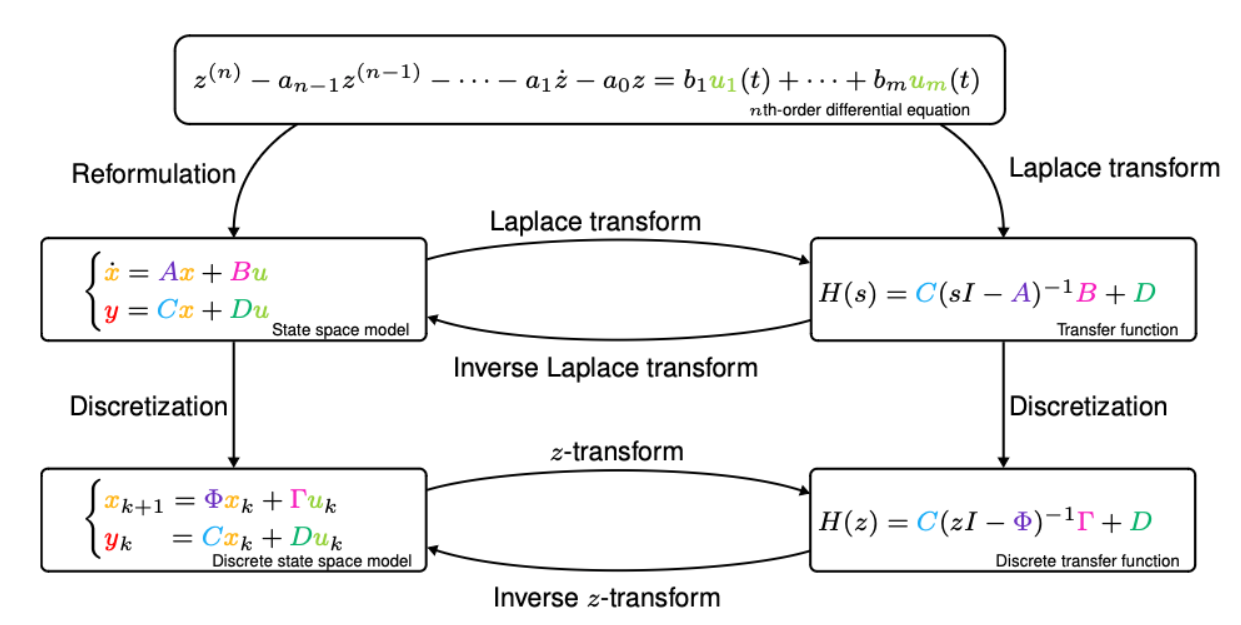
\includegraphics[width=0.9\textwidth]{Images/Models.png}
\end{center}
\subsection{Time-Domain models}
Two types of linear time-domain models. \\
Continous-time state space models
(based on differential equations)
$$\dot{x} = Ax+Bu$$
$$y=Cx+Du$$
\begin{itemize}
  \item $x\in \mathbb{R}^n$ is state
  \item $u\in \mathbb{R}^m$ is input
  \item $y\in \mathbb{R}^p$ is output
  \item $A\in \mathbb{R}^{n\times n}$ is system matrix
  \item $B\in \mathbb{R}^{n\times m}$ is input matrix
  \item $C\in \mathbb{R}^{p\times n}$ is output matrix
  \item $D\in \mathbb{R}^{p\times m}$ is the direct feedthrough matrix
\end{itemize}
Discrete-time state space models (based on difference equations)
$$x_{k+1} = \Phi x_k + \Gamma u_k$$
$$y_k = Cx_k + Du_k$$

\subsection{Frequency-Domain models}
Transfer function:
$$G(s)=\frac{Q(s)}{P(s)}$$
where $Q(s)$ and $P(s)$ are polynomials in $s$.
\begin{itemize}
  \item The roots of $P(s)$ are called the \textbf{poles} of $G(s)$
  \item The roots of $Q(s)$ are called the \textbf{zeros} of $G(s)$
\end{itemize}
\subsubsection{State space to transfer function}
Taking Laplace tranforms of the system and assuming $x_0=0$:
$$\dot{x}(t)=Ax(t)+Bu(t)$$
$$y(t)=Cx(t)+Du(t)$$
yields:
$$sX(s)=AX(s)+BU(s)$$
$$Y(s)=CX(s)+DU(s)$$
Which can be rewritten as ($I$ is the identity matrix):
$$X(s)=\left(sI-A\right)^{-1}BU(s)$$
$$Y(s)=\left(C\left(sI-A\right)^{-1}B+D\right)U(s)$$
where
$$Y(s)=G(s)U(s)$$
$$G(s)=C\left(sI-A\right)^{-1}B+D$$
\subsubsection{Transfer function to state space}

\subsubsection{Discrete-time transfer function}
Discretization from $s$-domain to $z$-domain can be done using:
\begin{itemize}
  \item Matched z-transform
  \item Bilinear z-transform
  \item Impulse invariance z-transform
\end{itemize}
\begin{center}
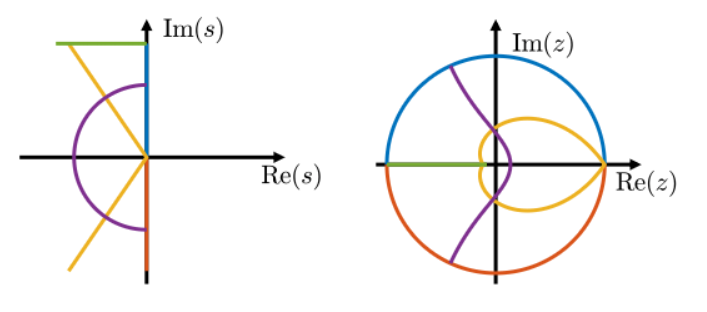
\includegraphics[width=0.6\textwidth]{Images/s-to-z.png}
\end{center}

\subsection{Examples}

